% !TEX root = fce.tex
% -----------------------------------------------------------------
% Filename  :	task4.tex
% Author    :	Carsten Hoppe
% Date		:	30. January 2017
% Reference	:	http://www.texample.net/tikz/examples/state-machine/
%				https://martin-thoma.com/how-to-draw-a-finite-state-machine/
% -----------------------------------------------------------------
In the following section we describe an implementation of an instruction cache and a data cache. We develop a \textit{Direct Mapped Cache} using as the instruction cache and a \textit{2-way set associative cache} using as the data cache.\\
At first we give a short introduction to memories \ref{sec:introductionToMemories}. After that, we simulate the efficiency of a cache with MARS in subsection \ref{sec:cacheSimulation} and compare different kinds of cache organizations. Afterwards, we design and implement a direct mapped cache in subsection \ref{sec:designDirectMappedCache}. This direct mapped cache will be used to develop a complete cache used as an instruction cache. Therefore, we design a finite state machine representing the behavior of this cache in \ref{sec:designFSMCache} and finally we write a testbench to verify the implementation in \ref{sec:testbenchSimulationCache}. 


\subsection{Introduction to Memories}
\label{sec:introductionToMemories}
TODO
Why are there so many different storage types?


A cache is a faster but smaller storage system which is placed nearby the CPU. In the Harvard architecture there is one cache for instructions and one cache for data. There are diverse modes to organize the caches. Primary, the caches are organized by answering the following four questions:
\begin{enumerate}
	\item \textit{Block Placement} - Where can a block be placed in the cache?
	\item \textit{Block Identification} - How is a block found in the cache?
	\item \textit{Block Replacement} - Which block is replaced in case of a cache miss?
	\item \textit{Write Strategies} - What happens during a write operation?
\end{enumerate}
So, there are different cache organizations. But what are the advantages and disadvantages of the different cache organization forms?\\
Regarding the \textit{Block Placement} there are three essential block placement strategies: \textit{Direct Mapped}, \textit{Set Associative} and \textit{Fully Associative}. The advandtage of the increasing of the grade of associativity is that the miss rate is reduced and the hit rate is increased. The disadvantage of the associativity is the complex implementation and slower access time.\\
In view of the \textit{Block Identification}increased
With respect to \textit{Block Replacement} either the \textit{LRU} strategy or the \textit{Random} strategy is used.\\ 
Regarding the \textit{Write Strategies} we distinguish between the \textit{Write-through} and \textit{Write-back} strategies. The advantages of the strategy Write-back is that single words can be written with the speed of the CPU and not of the main memory. Also, only one single write operation to the main memory is needed for multiple write operations. The advantages of the strategy Write-through are that cache misses can be simpler and cheaper handled. Eventually, the cache blocks do not needed to write back to the main memory in case of a cache miss. Furthermore, the strategy Write-through is easily to implemented.



\subsection{Cache Simulation - Results}
\label{sec:cacheSimulation}
In the following step we simulate the efficiency of a cache with MARS. On this, we compare the cache performance for different block sizes of a direct mapping cache, a 2-way associative cache and a 4-way associative cache. The two assembler programs \textit{row-major.asm} and \textit{column-major.asm} has been used for the cache simulation. For the simulation we vary the block size and placemet policy, but we fix the number of cache blocks to 8. Table \ref{tab:tableColumnMajor} contains the results regarding the file \textit{column-major.asm} and table \ref{tab:tableRowMajor} illustrates the results of \textit{row-major.asm}. The efficiency of a cache is evaluated by counting the number of cache hits and cache misses during executing the assembler program. Besides, the cache hit rate is determined by the cache hit count and the memory access count. In both assembler programs a 16x16 matrix is fully traversed. Therefore, we get a memory access count with value 256 for each program execution.\\
The first assembler program \textit{column-major.asm} traverses the 16x16 matrix column by column. At first we traverse the lead column, then the second column and so on. When we traverse the first half of a column, each correspondent block is loaded into the cache. But when we handle the second half of a column, the all data in the cache are replaced because all eight cache blocks are already occupied. In the next colum we also traverse at first the first half and then the second half of the column. When traversing the first half, we must also replace all data in the cache, because all cache blocks are already occupied and have different tag values. Finally, we expect that no cache hit occurs. In fact during each access to an array element causes a cache miss. As you can see in table \ref{tab:tableColumnMajor}, for all combinations of the placement policy and the cache block size we achieve a cache hit rate of zero.\\
Contrary to the column major program, we traverse the 16x16 matrix row by row. When we access an array element, the correspondent block is placed into the cache. Directly after accessing this element, we also access the nearby array elements of this block. Thus, we only expect one cache miss for the access of the first block element and cache hits  for accessing the remainding elemenets of a block. Depending on the cache block size (i.e. the number of words in a cache block), we achieve expect a diverse number of cache hit count and miss hit count. Moreover, table \ref{tab:tableRowMajor} shows that the results are equal relating to the placement policy.\\
The above assembler programs contrast traversing the matrix column by column with traversing row by row. Two principles of the cache memory are the \textit{Temporal Locality} and the \textit{Spatial Locality}. The above assembler programs illustrate the spatial locality. Thus, memory accesses whose addresses are adjacent will often be accessed in the near future. Therefore, the matrix is stored in memory row by row. The spatial locality requires to access contiguous data in memory element wise. Hence, it is efficient to traverse the given matrix row by row.

% Show table with simulation of column major assembler program.
\cacheTable{Cache Simulation of Column Major}{tab:tableColumnMajor}{
Direct Mapping & 2 & 0 & 256 & 0  \\
Direct Mapping & 4 & 0 & 256 & 0  \\
Direct Mapping & 8 & 0 & 256 & 0  \\
Direct Mapping & 16 & 0 & 256 & 0  \\
2-Way Set Associative & 2 & 0 & 256 & 0 \\
2-Way Set Associative & 4 & 0 & 256 & 0 \\
2-Way Set Associative & 8 & 0 & 256 & 0 \\
2-Way Set Associative & 16 & 0 & 256 & 0 \\
4-Way Set Associative & 2 & 0 & 256 & 0 \\
4-Way Set Associative & 4 & 0 & 256 & 0 \\
4-Way Set Associative & 8 & 0 & 256 & 0 \\
4-Way Set Associative & 16 & 0 & 256 & 0 \\}

% Show table with simulation results of row major assembler program.
\cacheTable{Cache Simulation of Row Major}{tab:tableRowMajor}{Direct Mapping & 2 & 128 & 128 & 50  \\
Direct Mapping & 4 & 192 & 64 & 75  \\
Direct Mapping & 8 & 224 & 32 & 88  \\
Direct Mapping & 16 & 240 & 16 & 94  \\
2-Way Set Associative & 2 & 128 & 128 & 50 \\
2-Way Set Associative & 4 & 192 & 64 & 75 \\
2-Way Set Associative & 8 & 224 & 32 & 88 \\
2-Way Set Associative & 16 & 240 & 16 & 94 \\
4-Way Set Associative & 2 & 128 & 128 & 50 \\
4-Way Set Associative & 4 & 192 & 64 & 75 \\
4-Way Set Associative & 8 & 224 & 32 & 88 \\
4-Way Set Associative & 16 & 240 & 16 & 94 \\}

\newpage
\subsection{Design a direct mapped cache}
\label{sec:designDirectMappedCache}
To develop an instruction cache and a data cache, we first implement a direct mapped cache. Thus, in figure \ref{fig:entityDirectMappedCache} we illustrate the entity of the direct mapped cache with all input and output ports.\\
Of course, the clock signal \textit{clk} is used to handle the behavior of this entity. The \textit{reset} signal is used to reset the direct mapped cache. When the direct mapped cache is reset, all cache block lines will become invalid. The input port \textit{addrCPU} stores the address given from the CPU to the cache. This address determines the cache block line to be read or to be written. The two inout ports \textit{dataCPU} and \textit{dataMEM} are needed to pass data word between the CPU and the cache as well as between the main memory and the cache. The input signal \textit{newCacheBlockLine} stores the new cache block line to be written into the direct mapped cache. Also, there are several control signals to specify, whether the direct mapped cache should be written or read. The signals \textit{wrCBLine} and \textit{rdCBLine} states whether a whole cache block line should be written or read. Accordingly, the signals \textit{rdWord} and \textit{wrWord} satisfy whether a single word should be written or read in the direct mapped cache. The control signal \textit{wrNewCBLine} says, whether a new cache block line should be written into the direct mapped cache. Furthermore, the input ports \textit{setValid} and \textit{setDirty} controls whether the dirty bit and the valid bit should be reset. The inout port \textit{dirty} stores the new value of the dirty bit or the returns the current value of the dirty bit regarding the current cache block line. Finally, the out port \textit{hit} signalises whether a cache hit or a cache miss is achieved during a read/write operation.

% Figure of entity of the Direct Mapped Cache.
\begin{figure}[htb]
\label{fig:entityDirectMappedCache}
\centering
\begin{tikzpicture}[font=\sffamily,>=triangle 45]
  \node [shape=circuit] (item) at (0,0) {directMappedCache};
  \draw [<-] (item.ina) node [anchor=west,labels] {} -- +(-1,0) node [anchor=east] {clk};
  \draw [<-] (item.inb) node [anchor=west,labels] {} -- +(-1,0) node [anchor=east] {reset};
  \draw [<-] (item.inc) node [anchor=west,labels] {} -- +(-1,0) node [anchor=east] {addrCPU};
  \draw [<->] (item.ioa) node [anchor=east,labels] {} -- +(1,0) node [anchor=west] {dataCPU};
  \draw [<-] (item.ind) node [anchor=west,labels] {} -- +(-1,0) node [anchor=east] {newCacheBlockLine};
  \draw [<->] (item.iob) node [anchor=east,labels] {} -- +(1,0) node [anchor=west] {dataMEM};
  \draw [<-] (item.ine) node [anchor=west,labels] {} -- +(-1,0) node [anchor=east] {wrNewCBLine};
  \draw [<-] (item.inf) node [anchor=west,labels] {} -- +(-1,0) node [anchor=east] {wrCBLine};
  \draw [<-] (item.ing) node [anchor=west,labels] {} -- +(-1,0) node [anchor=east] {rdCBLine};
  \draw [<-] (item.inh) node [anchor=west,labels] {} -- +(-1,0) node [anchor=east] {rdWord};
  \draw [<-] (item.ini) node [anchor=west,labels] {} -- +(-1,0) node [anchor=east] {wrWord};
  \draw [<-] (item.inj) node [anchor=west,labels] {} -- +(-1,0) node [anchor=east] {writeMode};
  \draw [->] (item.outa) node [anchor=east,labels] {} -- +(1,0) node [anchor=west] {hit};
  \draw [<->] (item.ioc) node [anchor=east,labels] {} -- +(1,0) node [anchor=west] {dirty};
  \draw [<-] (item.ink) node [anchor=west,labels] {} -- +(-1,0) node [anchor=east] {setValid};
  \draw [<-] (item.inl) node [anchor=west,labels] {} -- +(-1,0) node [anchor=east] {setDirty};
\end{tikzpicture}
\caption{Entity of directMappedCache}
\end{figure}


\newpage
\subsection{Design a Finite State Machine for the Cache}
\label{sec:designFSMCache}
% !TEX root = task4.tex
% -----------------------------------------------------------------
% Filename  :	task4_stateMachine_writeAllocatePolicy.tex
% Author    :	Carsten Hoppe
% Date		:	28. Januar 2017
% Reference	:	http://www.texample.net/tikz/examples/state-machine/
%				https://martin-thoma.com/how-to-draw-a-finite-state-machine/
% -----------------------------------------------------------------
%\tikzstyle{every state}=[fill=mycolor,text=white,minimum width=2cm]
After we have implemented the direct mapped cache, we have to design a finite state machine for the cache controller. This controller have to count the cache hits and cache misses using counters, which are reset at program start. On the one hand, we implement the write back policy. On the other hand, we implement the write allocate policy.\\
In figure \ref{tik:FSM} the state diagram of the cache controller is illustrated. The state diagram represents a Mealy automaton. Besides the state machine inputs are listed in table \ref{tab:tableFSMInputs} and the state machine outputs are shown in table \ref{tab:tableFSMOutputs}. A sketch of the state diagram is printed in figure \ref{fig:sketchMealyAutomata}.\\
In the following, we describe the state space of the state machine:
\begin{itemize}
	\item[IDLE] This state is the initial state of the state machine. When the cache is reset and state machine switches to this state.
	\item[CHECK1] In this state, the cache is checking whether write operation will results in a cache hit or not. Thus, the valid bit, dirty bit and the tag values of the correspondent cache block line are relevant for checking cache hit or cache miss.
	\item[CHECK2] In this state, the cache is checking whether read operation will results in a cache hit or not. Thus, the valid bit, dirty bit and the tag values of the correspondent cache block line are relevant for checking cache hit or cache miss.
	\item[WRITEBACK1] When checking the current cache block line results in a cache miss, and the current cache block line is dirty, this cache block line must be written back to the main memory first. Inside this state, the cache writes the cache block line back to the main memory. The process of writting back requires a specific number of clock cycles. Thus, we have to wait for the main memory. If the main memory signalizes that it is ready, then we can change this state to the next state.
	\item[WRITEBACK2] When checking the current cache block line results in a cache miss, and the current cache block line is dirty, this cache block line must be written back to the main memory first. Inside this state, the cache writes the cache block line back to the main memory. This process of writting back requires a specific number of clock cycles. Thus, we have to wait for the main memory. If the main memory signalizes that it is ready, then we can change this state to the next state.
	\item[WRITE] Before we will write the new data word into the cache, we have to read the cache block line from the main memory into the cache. While the cache is reading from the main memory, we stay in this state. When the main memory is ready and the cache finished reading from the main memory, we switch the current state.
	\item[READ] In case of a cache miss, we have to read the correspondent cache block line from the main memory into the cache. While the we are reading from the main memory, we are inside this state. The main memory signalizes via a correspondent signal if the read operation is finished.
	\item[TOCACHE1] When the write operation has been finished, we achieve this state of the state machine. This state is necessary to increment the miss counter by one. 
	\item[TOCACHE2] When the read operation has been finished, we achieve this state. This state is necessary to increment the miss counter by one. Also, we transmit the requested data word from the cache to the CPU.
\end{itemize}


\newpage
\begin{landscape}
\begin{figure}
	\centering
	\caption{State diagram of the cache controller.}
    \label{tik:FSM}
	\fcolorbox{blue}{myOrange}{
	\begin{tikzpicture}[->,>=stealth',shorten >=1pt,auto,semithick,/tikz/initial text=Reset]
                    
	% ------------------------------------------------------------------------------
    % Definition of tikz styles.       
	% ------------------------------------------------------------------------------
	\tikzstyle{vertex}=[state,fill=mycolor,text=white,minimum width=1cm]
	\tikzstyle{edge}  =[draw,thick,->, midway, above, sloped, font=\tiny]
	\tikzset{invisible/.style={minimum width=0mm,inner sep=0mm,outer sep=0mm}}
	
	% ------------------------------------------------------------------------------
	% Definition of nodes.
	% ------------------------------------------------------------------------------
	[align=center,xscale=1,node distance=2cm and 4cm]
	\node[initial,vertex]	(A)                    		{\tiny $IDLE$};
  	\node[vertex]         	(B) [below  left=5cm of A] 	{\tiny $CHECK1$};
  	\node[vertex]			(C) [below right=5cm of A]	{\tiny $CHECK2$};
  	\node[vertex]         	(D) [below  left=4cm of B] 	{\tiny $WRITEBACK1$};
  	\node[vertex]         	(E) [below right=4cm of C] 	{\tiny $WRITEBACK2$};
  	\node[vertex]         	(F) [below right=4cm of D] 	{\tiny $WRITE$};
  	\node[vertex]			(G) [below  left=4cm of E]  {\tiny $READ$};
  	\node[vertex]		    (H) [below  =2cm of F]  {\tiny $TOCACHE1$};
  	\node[vertex]			(I) [below =2cm of G]  {\tiny $TOCACHE2$};
  	\node	(J) [below =9cm of A,invisible]	{};

	% ------------------------------------------------------------------------------
	% Definition of paths.
	% ------------------------------------------------------------------------------
	\path (A) [edge] 	edge [bend right] node 	{wrCPURequest/-} 	(B)
	      (A) [edge]	edge [bend  left] node  {rdCPURequest/-}	(C)
	      (B) [edge]	edge [bend right] node  {hit/hitCounter++, data2Cache} (A)
	      (C) [edge]	edge [bend left ] node  {hit/hitCounter++, data2CPU} (A)
	      (B) [edge]    edge [bend left ] node  {lineIsNotDirty / rdMEM='1'} (F)
	      (B) [edge]    edge [bend right] node  {lineIsInvalid / rdMEM='1'} (F)
	      (B) [edge]	edge			  node	{lineIsDirty / cacheLine2MEM} (D)
	      (D) [edge]	edge 			  node	{readyMEM / rdMEM='1'} (F)
	      (F) [edge]	edge			  node	{readyMEM / wrNewCBLine} (H)
	      (H) [edge] 	edge [bend right] node 	{- / missCounter++, data2Cache} (J)
	      (C) [edge]	edge 			  node  {lineIsDirty / cacheLine2MEM} (E)
	      (C) [edge]	edge [bend right] node  {lineIsInvalid / rdMEM='1'} (G)
	      (C) [edge]	edge [bend left ] node  {lineIsNotDirty / rdMEM='1'} (G)
	      (E) [edge]	edge 			  node	{readyMEM / -} (G)
	      (I) [edge]	edge [bend left ] node	{- / missCounter++, data2CPU} (J)
	      (G) [edge]	edge 			  node  {readyMEM / -} (I)
	      (J) [edge]	edge 			  node  {} (A)
	      (E) [edge,loop right] edge	  node  {!readyMEM / -} (E)
	      (G) [edge,loop left]  edge	  node  {!readyMEM / -} (G)
	      (D) [edge,loop left] edge 	  node	{!readyMEM / -} (D)
	      (F) [edge,loop right] edge	  node  {!readyMEM / -} (F);
	      		
\end{tikzpicture}}
\end{figure}
\end{landscape}
\newpage

\begin{table}
	\caption{Overview - FSM Inputs}
	\label{tab:tableFSMInputs}
	\begin{tabular}{lll}
	\hline % \topline
	Abbreviation & Name & Description \\
	\hline % \midrule
	rdCPU 		& CPU Read Request			& - \\
	wrCPU 		& CPU Write Request 		& - \\
	cacheMiss 	& Cache Miss 				& - \\
	cacheHit	& Cache Hit					& - \\
	readyMEM 	& Write-Back is resolved 	& - \\
	isDirty		& Cache Block is dirty		& - \\
	\hline % \bottomrule
	\end{tabular}
\end{table}
	
\begin{table}
	\caption{Overview - FSM Outputs}
	\label{tab:tableFSMOutputs}
	\begin{tabular}{lll}
	\hline % \topline
	Abbreviation & Name & Description \\
	\hline % \midrule
	stallCPU		& Stall Processor				& - \\
	setDirty		& Set Dirty Bit (Modified) Bit 	& - \\
	wrMEM			& Write To Memory				& Write Replaced Block To Memory \\
	dataCPU			& Read Data Into CPU			& - \\
	rdMEM			& Read Cache Block Into Cache From Memory & - \\
	dataCPU2Cache	& Write Data Into Cache			& - \\
	\hline % \bottolrule
	\end{tabular}
\end{table}

\newpage
\begin{landscape}
\begin{figure}
	\centering
	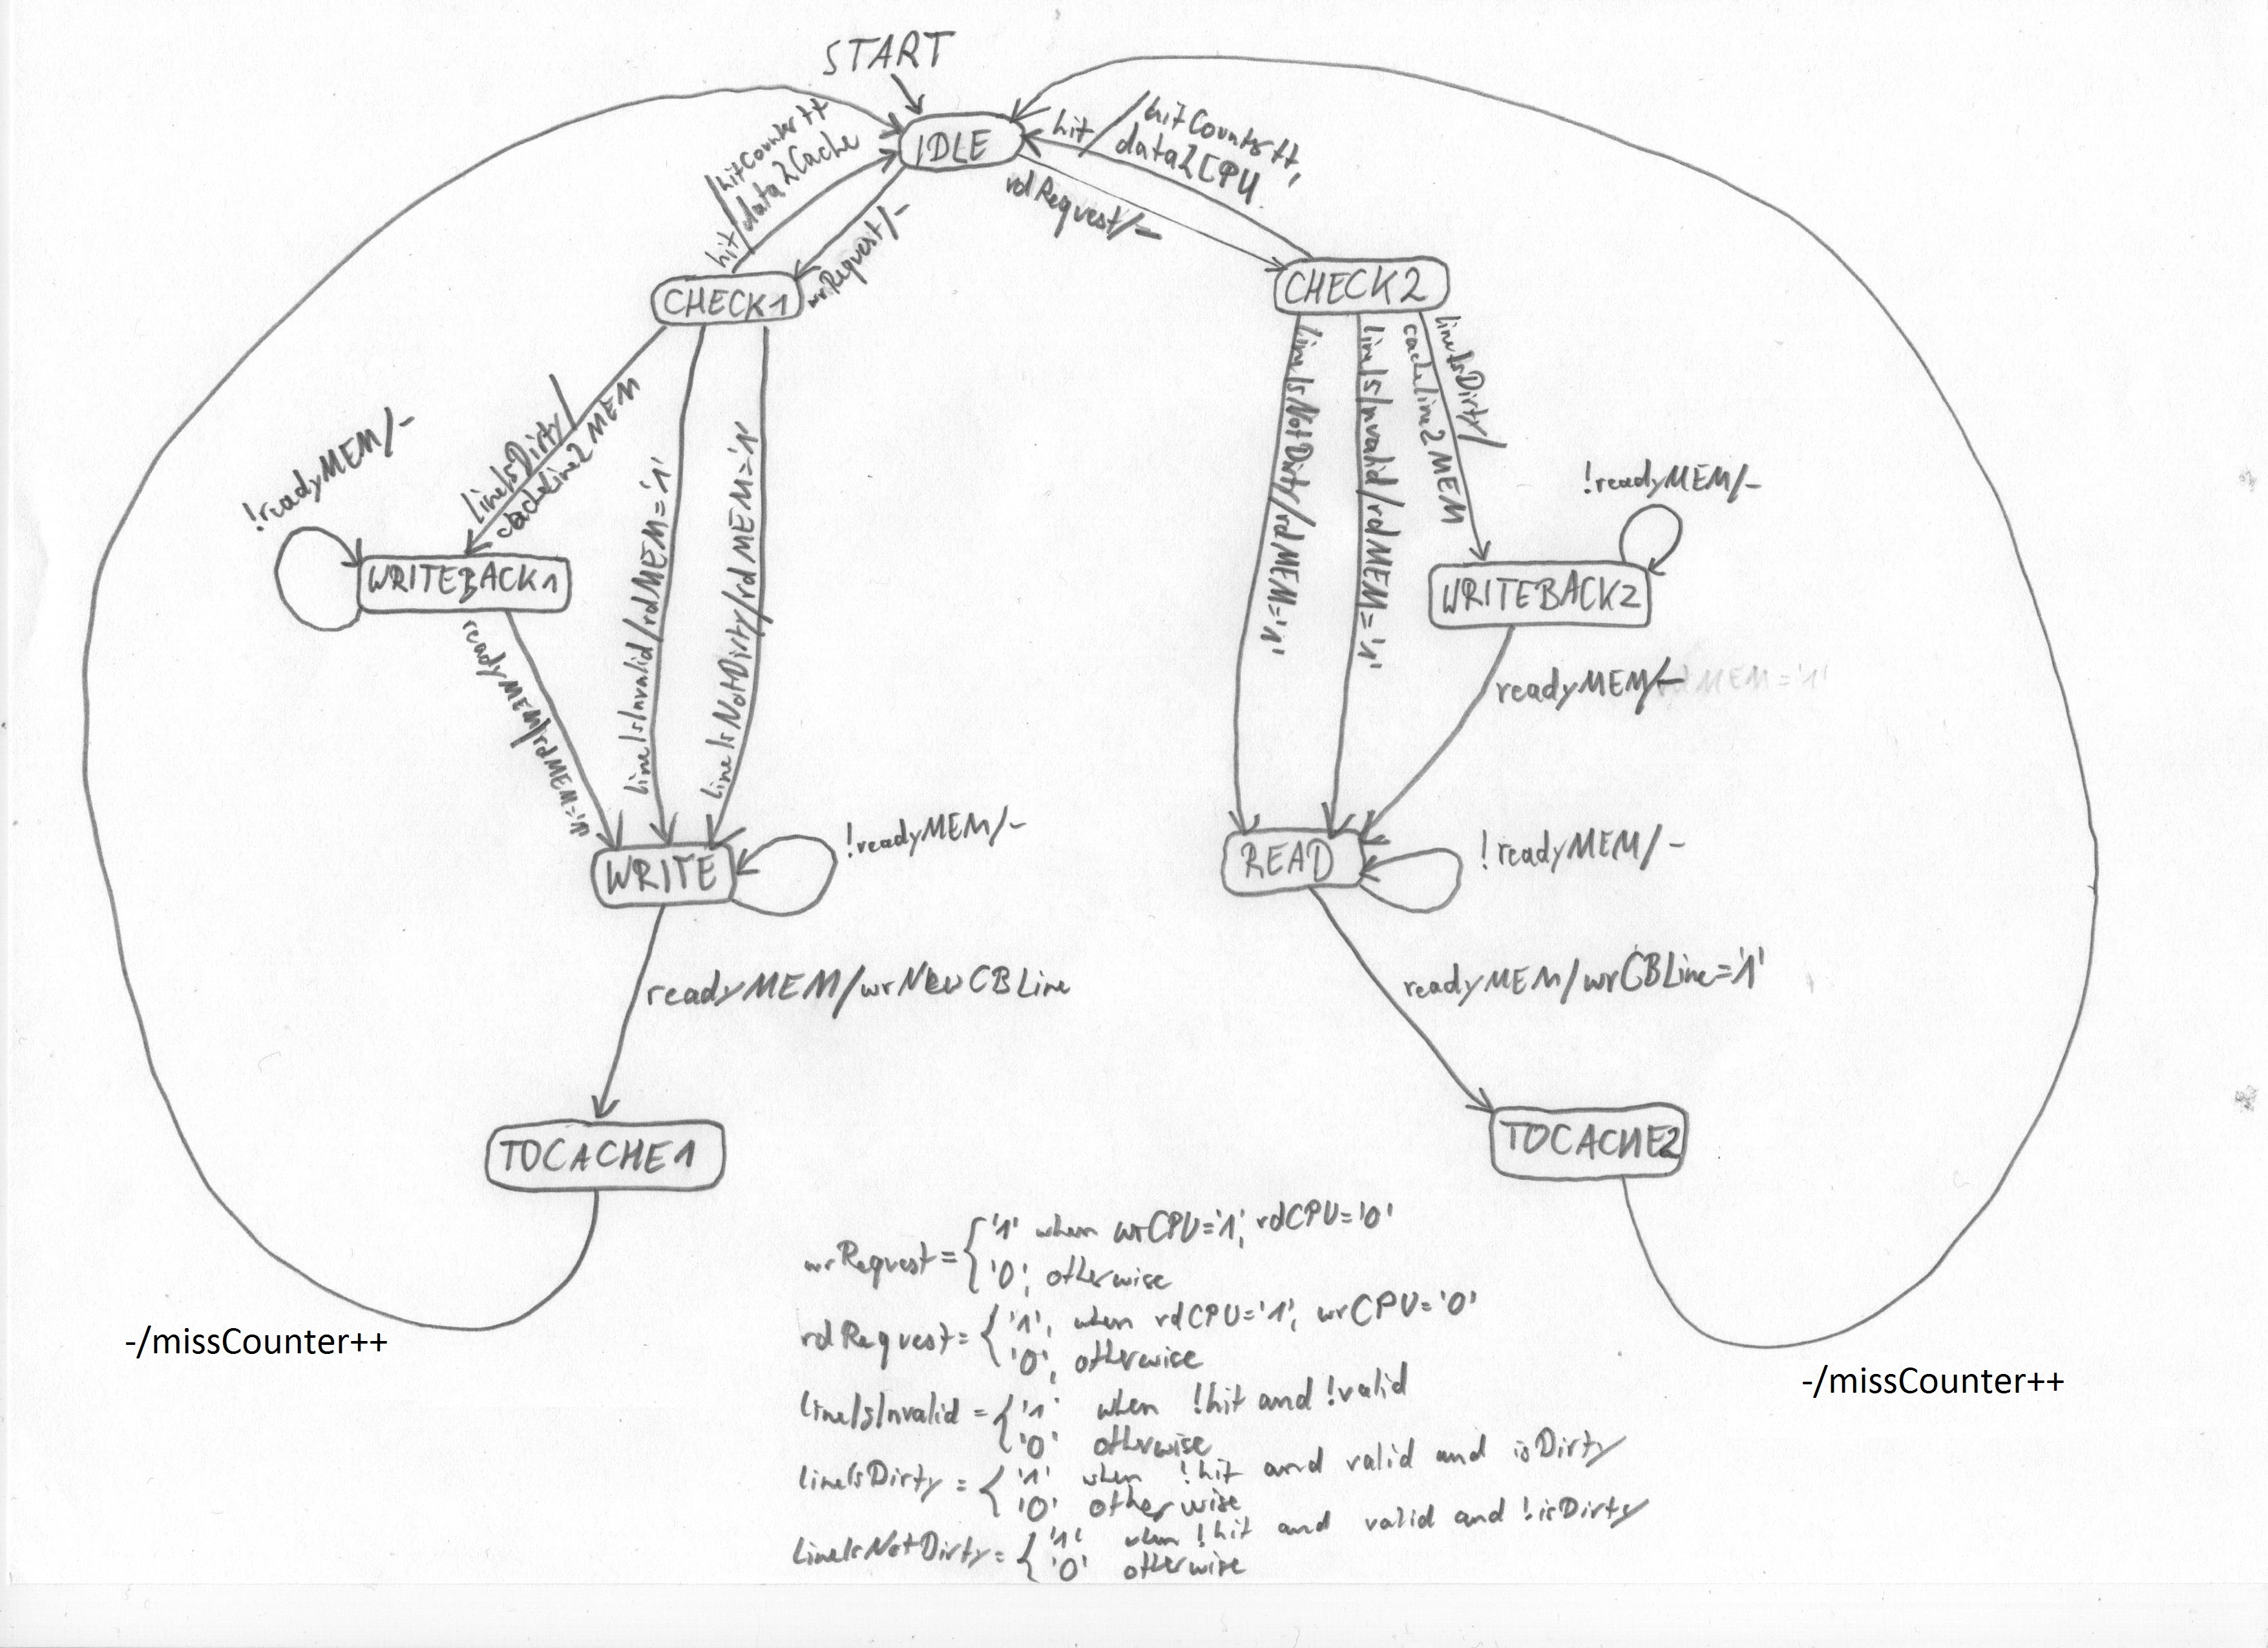
\includegraphics[scale=.8]{pictures/sketch_mealyAutomata_v2_modified}
	\caption{Sketch of Mealy Automata - Cache Controller, Version 2}
	\label{fig:sketchMealyAutomata}
\end{figure}
\end{landscape}

\newpage
\subsubsection{Design a Finite State Machine for the Main Memory Controller}
The main memory controller has the purpose to either write a given cache block/line to the main memory or to read multiple words from the main memory and return these words as a cache block/line. This main memory controller will be connected with the cache controller. Thus, the main memory controller will send a read cache block/line from the main memory to the cache controller. Also the main memory will get a cache block/line from the cache controller, which should be written into the main memory. Consider that a single data word has a certain wide of bits and a whole cache block/line contains several data words. Furthermore, the main memory could be implemented as a BlockRAM (BRAM). At first, the main memory controller is implemented as a finite state machine of type Mealy. The sketch of the finite state machine is given in figure~\ref{tik:FSM_MainMemory}.


\newpage
\begin{figure}
	\centering
	\caption{Sketch of Mealy Automata - Main Memory Controller}
    \label{tik:FSM_MainMemory}
	\begin{tikzpicture}[->,>=stealth',shorten >=1pt,auto,semithick,/tikz/initial text=Reset]
                    
	% ------------------------------------------------------------------------------
    % Definition of tikz styles.       
	% ------------------------------------------------------------------------------
	\tikzstyle{vertex}=[state,fill=mycolor,text=white,minimum width=1cm]
	\tikzstyle{edge}  =[draw,thick,->, midway, above, sloped, font=\tiny]
	\tikzset{invisible/.style={minimum width=0mm,inner sep=0mm,outer sep=0mm}}
	
	% ------------------------------------------------------------------------------
	% Definition of nodes.
	% ------------------------------------------------------------------------------
	[align=center,xscale=1,node distance=2cm and 4cm]
	\node[initial,vertex]	(A)                    		{\tiny $IDLE$};
  	\node[vertex]         	(B) [below  left=5cm of A] 	{\tiny $READ$};
  	\node[vertex]			(C) [below right=5cm of A]	{\tiny $WRITE$};
  	\node[vertex]         	(D) [below =10cm of A] 		{\tiny $DELAY$};

	% ------------------------------------------------------------------------------
	% Definition of paths.
	% ------------------------------------------------------------------------------
	\path (A) [edge] 	edge node  {rdRequest / counter=0} 	(B)
	      (A) [edge]	edge node  {wrRequest / counter=0}	(C)
	      (B) [edge]	edge node  { counter$>$BLOCKSIZE /  } (D)
	      (C) [edge]	edge node  { counter$\geq$BLOCKSIZE / } (D)
	      (D) [edge]    edge node  { counter$\geq$20 / } (A)
		  (B) [edge,loop left] edge	  node  { counter$\leq$BLOCKSIZE / counter++ } (B)	
		  (C) [edge,loop right] edge	  node  { counter$<$BLOCKSIZE / counter++} (C)
		  (D) [edge,loop below] edge	  node  { counter$<$20 / counter++} (D)	      
	      
	      ;
	      
	      
%	      (B) [edge]    edge [bend right] node  {lineIsInvalid / rdMEM='1'} (F)
%	      (B) [edge]	edge			  node	{lineIsDirty / cacheLine2MEM} (D)
%	      (D) [edge]	edge 			  node	{readyMEM / rdMEM='1'} (F)
%	      (F) [edge]	edge			  node	{readyMEM / wrNewCBLine} (H)
%	      (H) [edge] 	edge [bend right] node 	{- / rMissCt++, data2Cache} (J)
%	      (C) [edge]	edge 			  node  {lineIsDirty / cacheLine2MEM} (E)
%	      (C) [edge]	edge [bend right] node  {lineIsInvalid / rdMEM='1'} (G)
%	      (C) [edge]	edge [bend left ] node  {lineIsNotDirty / rdMEM='1'} (G)
%	      (E) [edge]	edge 			  node	{readyMEM / -} (G)
%	      (I) [edge]	edge [bend left ] node	{- / rMissCt++, data2CPU} (J)
%	      (G) [edge]	edge 			  node  {readyMEM / -} (I)
%	      (J) [edge]	edge 			  node  {} (A)
%	      (E) [edge,loop right] edge	  node  {!readyMEM / -} (E)
%	      (G) [edge,loop left]  edge	  node  {!readyMEM / -} (G)
%	      (D) [edge,loop left] edge 	  node	{!readyMEM / -} (D)
%	      (F) [edge,loop right] edge	  node  {!readyMEM / -} (F);
	      		
\end{tikzpicture}
\end{figure}


\newpage
\subsection{Design a testbench and simulate the Cache}
\label{sec:testbenchSimulationCache}
After implementation of the Cache with \textit{Write Back Policy} and \textit{Write Allocate Policy} we write a testbench and simulate a system with the following properties:
\begin{itemize} 
	\item Main memory using a BlockRAM with ready signal.
	\item Direct Mapped Cache with 256 blocks/lines. Each block/line has 4 words. The cache use the write back scheme. Also, byte access is possible.	
\end{itemize}
The testbench should verify the behavior of the cache. Therefore, we look at different test cases. In the following table \ref{tab:testCases} we describe some test cases.\\
We have created the batch file \textit{test\_cacheTestbench.bat} to run the testbench with GHDL. Thus, we start the simulation by typing \textit{test\_cacheTestbench.bat} in the command-line user interface. Figure \ref{fig:simulationResult} shows that all test cases are successfully executed.\\
When illustrating the simulation results in Gtkwave, the number of clock cycles needed for a cache hit and cache miss can be determined. As you can see in figure \ref{fig:simulationResultCacheHit}, circa 6 clock cycles are needed for a cache hit.
\begin{figure}
	\centering
	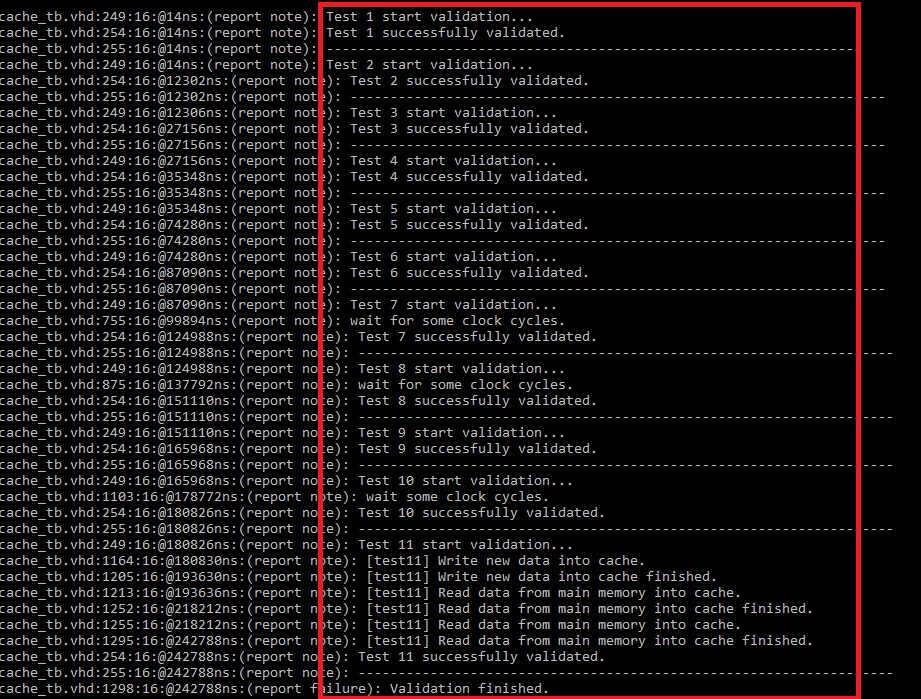
\includegraphics[scale=.5]{pictures/simulationResult}
	\caption{Result Simulation - Cache}
	\label{fig:simulationResult}
\end{figure}
\begin{figure}
	\centering
	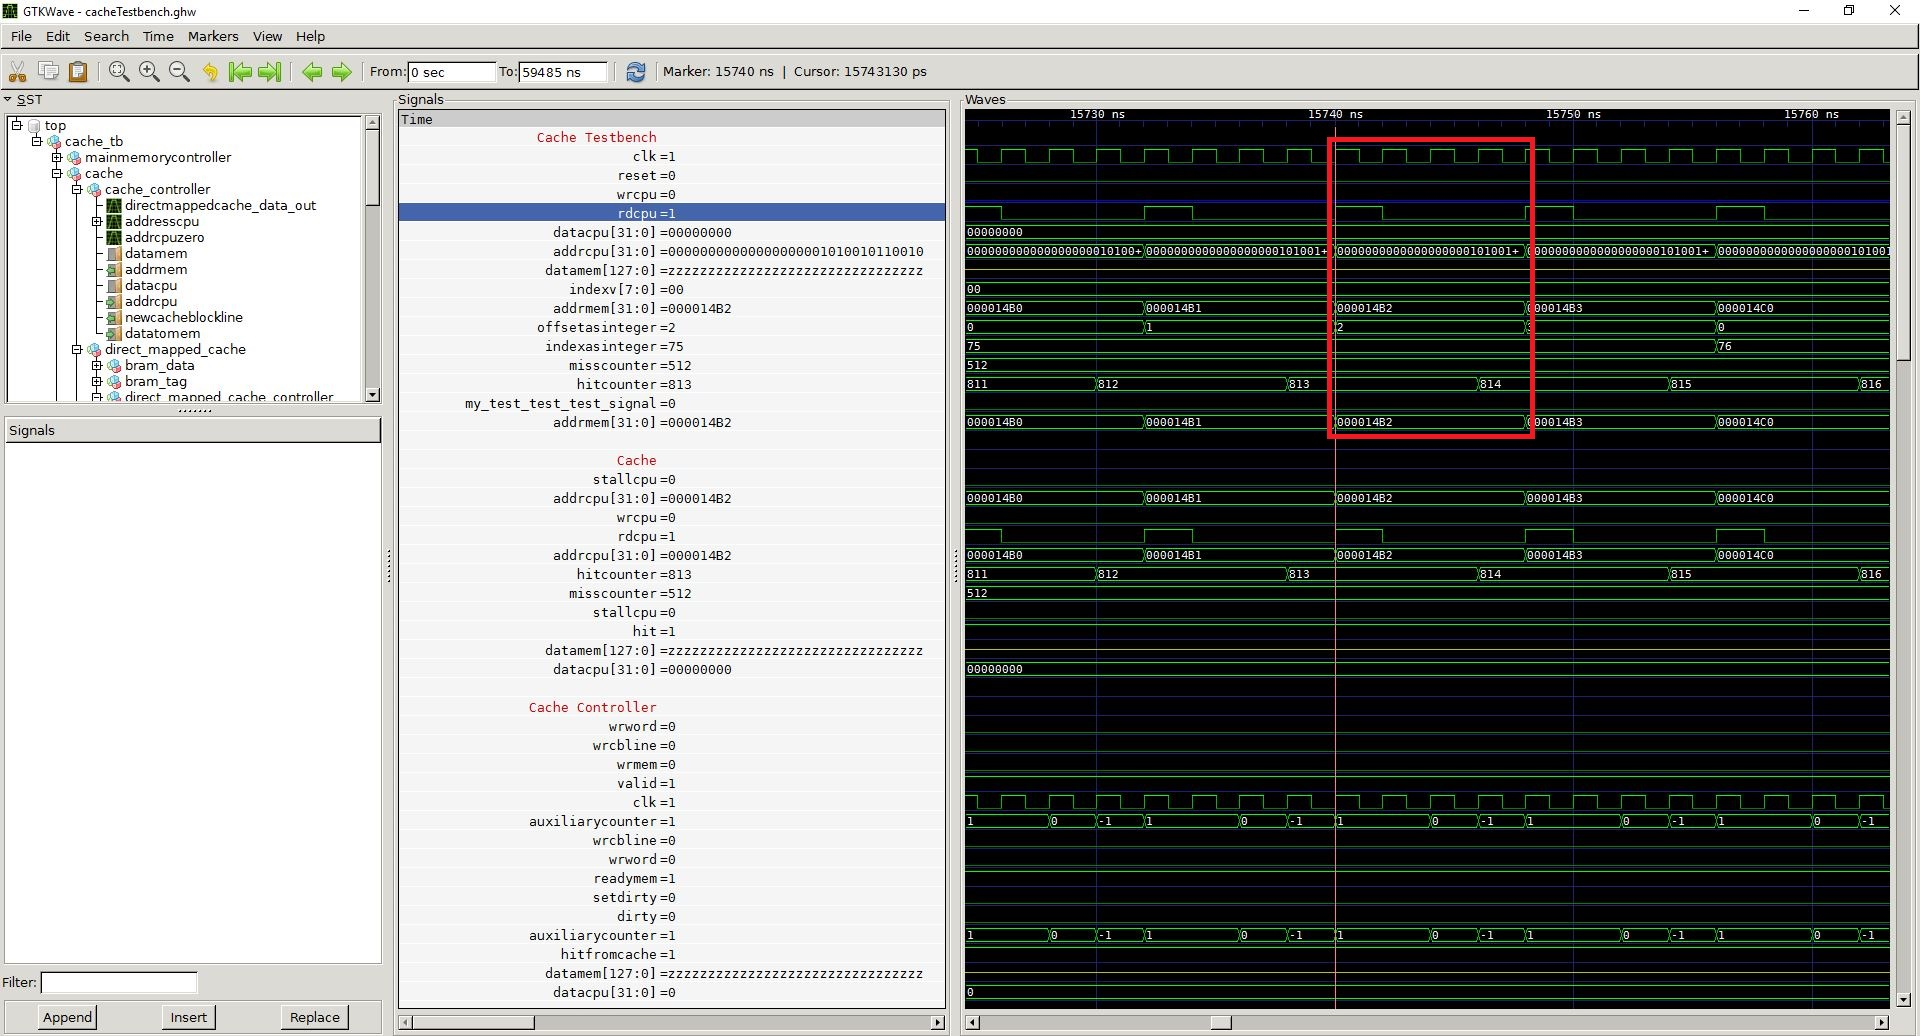
\includegraphics[scale=.4]{pictures/simulationResultGTKWaveCacheHit}
	\caption{Result Simulation Gtkwave - Cache Hit}
	\label{fig:simulationResultCacheHit}
\end{figure}

\begin{table}
\caption{Test Cases for Simulation}
\label{tab:testCases}
\begin{tabular}{rl}

\rowTableTestCases{Test Case 1}{Reset Cache I}{If the cache is reset, then the miss counter and the hit counter are reset to zero.}

\rowTableTestCases{Test Case 2}{Reset Cache II}{If the cache is reset, then all cache blocks lines are invalid.}

\rowTableTestCases{Test Case 3}{Read Cache, Line Is Not Dirty}{Assume, that there are already valid data in the cache block lines. Also, the data are not modified against the main memory. Now we read again with different tag values. Thus, the data are directly read from main memory into the cache. We expect that the miss counter is incremented and the stall signal is set to one.}

\rowTableTestCases{Test Case 4}{Read Cache, Different Offset}{In the first step, we are going to read the first word from a cache block line. Following we read another word from the same cache block line. Thus, the miss counter will be incremented.}

\rowTableTestCases{Test Case 5}{Read Cache, Line is Dirty}{
There are already valid data words in the cache block line. Also, the data words are modified compared to the main memory. Now, we are going to read again from cache while the tag values are differen. Thus, we expect that the modified data words are written back to the main memory first. Afterwards the block is read from main memory into the cache. Hence, the miss counter will be incremented.}

\rowTableTestCases{Test Case 6}{Write Cache, Invalid Cacheblocks}{Initially all cache blocks are invalid. If a cache block line is read, then the equivalent block is read from the main memory to the cache. Appropriate the miss counter will be incremented and the stall signal is set to '1'.}

\rowTableTestCases{Test Case 7}{Write Cache – Line is Dirty}{Assume, that there are already valid data words in the cache block line. The data words are modified compared to the main memory. We are going to write again into the cache block lines whereupon the tag values are different. Hence, the data from the cache are written back to the main memory first. After that the correspondent main memory block is load into the cache with the new written data given from CPU. We expect that the miss counter is incremented.}

\rowTableTestCases{Test Case 8}{Write Cache, Line Is Not Dirty}{Let's assume that there are already valid, clean data in a cache block/line. If we write new data to this cache block/line and the tags are different, then the valid, clean data will not be written back to the main memory. Instead of that, the correspondent block are read from memory to cache and the relevant offset block is replaced with the new data word. We expect, that the miss counter will be incremented.}

\rowTableTestCases{Test Case 9}{Write Cache - Hit}{Let's assume that there are already valid (clean or invalid) data in the cache block line. If we write new data to this cache block/line and the tags are equal, then then the old data will not be written back to the main memory. Instead of that, the correspondent cache block line is directly rewritten with the new data word. We expect, that the hit counter is incremented.}

\rowTableTestCases{Test Case 10}{Write Cache - Check Values}{In this test case we will check whether the new data word has been successfully written into the cache. Whatever the current status of the cache block/line is, we write new data into cache in the first step. After we have finished writing the cache, we can read the cache block line again. We expect, that we read the equal data from the cache, which we have written into the cache before.}

\end{tabular} 
\end{table}
